\begin{figure}[H]
    \centering
    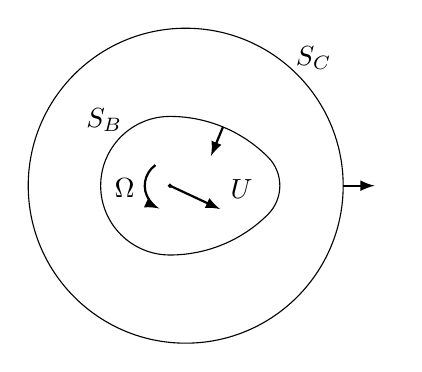
\begin{tikzpicture}
    \begin{scope}[scale = .4]
        \def\r{2.2}
        \def\R{5}
        \coordinate (O) at (0,0);
        \draw (0,\r) arc (90:270:\r)--(0,-\r) arc (270:315:{2*\r})--({\r*sqrt(2)}, {\r*(1-sqrt(2))}) arc (-45:45:{\r*(2-sqrt(2))})--({\r*sqrt(2)}, {\r*(sqrt(2)-1)}) arc (45:90:{2*\r});
        \node at ({(\r + .75)*cos(135)}, {(\r + .75)*sin(135)}) {$S_B$};
        \draw[-latex, thick] ({2*\r*cos(67.5)}, {2*\r*sin(67.5) - \r})--({(2*\r - 1)*cos(67.5)}, {(2*\r - 1)*sin(67.5) - \r}) node[midway, left]{$\nhat$};
        \draw[-latex, thick] (O)--({.8*\r*cos(-25)}, {.8*\r*sin(-25)}) node[above right]{$\bm{U}$};
        \draw[fill = black] (O) circle (.05);
        \def\rr{.8}
        \def\iangel{125} \def\fangel{245}
        \draw[-latex, thick] ({\rr*cos(\iangel)}, {\rr*sin(\iangel)}) arc (\iangel:\fangel:\rr) node[midway, left]{$\bm{\Omega}$};
        \def\disp{.5}
        \draw ({\disp}, {0}) circle (\R);
        \draw[-latex, thick] ({\R + \disp}, 0)--({\R + \disp + 1}, 0) node[right]{$\nhat$};
        \node at ({\disp + (\R + .75)*cos(45)}, {(\R + .75)*sin(45)}) {$S_C$};
    \end{scope}
\end{tikzpicture}
\end{figure}
We consider a submerged body in an unbounded fluid moving with velocity $\bm{U} = U(t)\ihat$.
The fluid is described by a potential $\Phi(\xvec, t)$, whose gradient is evanescent at large $r$.
Physically, this means that the motion of the body through the fluid does not influence the fluid in the far field.
We impose the kinematic boundary condition on the body of slip, meaning $\partial_{\nhat} \Phi = \bm{U}\cdot\nhat$, where $\nhat = n_x \ihat + n_y \jhat$.
As an ansatz, we say that
\[
    \Phi(\xvec, t) = U(t) \phi(\xvec),
\]
where $\phi(\xvec)$ satisfies the \textsc{Laplace} equation
\[
    \nabla^2 \phi = 0, \quad \text{in } \Omega,
\]
\[
    \partial_{\nhat} \phi = n_x, \quad \text{on } \partial\Omega,
\]
\[
    \lim_{r \to \infty} \absl{\nabla\phi} = 0,
\]
The very essence of this course is to predict the forces and moments acting on a body past which fluid motion flows.
By \textsc{Bernoulli}'s equation, we have that
\begin{equation*}
    \begin{aligned}
        \bm{F} & = \int_{S_B} p \nhat\,\dee S\\
        & = -\varrho\int_{S_B} \left(\deet\phi + \sfrac{1}{2}{\absl{\nabla\phi}}^2\right)\nhat \,\dee S,
    \end{aligned}
\end{equation*}
\begin{equation*}
    \begin{aligned}
        \bm{M} & = \int_{S_B} p \xvec\times\nhat \,\dee S\\
        & = -\varrho \int_{S_B} \left( \deet\phi + \sfrac{1}{2}{\absl{\nabla\phi}}^2 \right) \xvec\times\nhat \,\dee S.
    \end{aligned}
\end{equation*}
We now need the \textsc{Reynolds} transport theorem, which states that for a function of the form
\[
    I(t) = \int_{\Omega} f(\xvec, t) \,\dee V,
\]
its derivative is given by
\begin{equation}\tag{3.11}\label{eq:REYNOLDS_transport}
    I^{\prime}(t) = \int_{\Omega} \deet f \,\dee V + \int_{\partial\Omega} f \bm{U}\cdot\nhat \,\dee S,
\end{equation}
and the generalized \textsc{Stokes} theorem,
\begin{equation}\tag{4.85}\label{eq:generalized_STOKES}
    \int_{\Omega} \nabla f \,\dee V = \int_{\partial\Omega} f \nhat \,\dee S.
\end{equation}
The rate of change of the momentum of the volume enclosed by $S_C$ is given by
\[
    \varrho \frac{\dee}{\dee t}\int_{V} \nabla\phi \,\dee V = \varrho \frac{\dee}{\dee t}\int_{S_B + S_C} \phi \nhat \,\dee S.
\]
Using the \textsc{Reynolds} transport theorem on the left-hand side, and interchanging the gradient and temporal derivative, we have that it is equal to
\[
    \varrho \int_{\Omega} \nabla\deet\phi \,\dee V + \varrho \int_{\partial\Omega} \nabla\phi (\bm{U} \cdot \nhat) \,\dee S,
\]
Now using the genrealized \textsc{Stokes} theorem, we have that it further simplifies to
\[
    \varrho \int_{\partial\Omega} \deet \phi \nhat \,\dee S + \varrho \int_{\partial\Omega} \nabla\phi (\bm{U} \cdot \nhat) \,\dee S.
\]
Since the contour $S_B$ is steady, we may interchange the temporal differential operator with the integral for that contribution to $\partial\Omega$.
Due to impermeability, we have that $\bm{U} \cdot \nhat$ on that contour.
Furthermore, $\partial_{\nhat} \phi = \bm{U} \cdot \nhat$, so
\[
    \varrho \frac{\dee}{\dee t} \int_{S_B} \phi \nhat \,\dee S = \varrho \int_{S_B} \big( \deet\phi\nhat + \partial_{\nhat} \phi \nabla\phi \big) \,\dee S.
\]
We may rewrite the rate of change of the momentum, or the force, in terms of the above, we have that
\begin{equation*}
    \begin{aligned}
        \bm{F} = & - \varrho \frac{\dee}{\dee t} \int_{S_B} \phi \nhat \,\dee S\\
        & - \varrho\int_{S_C} \big( \partial_{\nhat} \phi \nabla\phi - \sfrac{1}{2}\absl{\nabla \phi}^2 \nhat \big) \,\dee S,
    \end{aligned}
\end{equation*}
where we have used that
\[
    \int_{\partial\Omega} \big( \partial_{\nhat}\phi \nabla\phi - \sfrac{1}{2}\absl{\nabla \phi}^2 \nhat \big) \,\dee S = \int_{\Omega} \nabla\phi \nabla^2 \phi \,\dee V \equiv 0.
\]
In a similar manner, one may use
\[
    \int_{\Omega} \nabla\times\bm{Q} \,\dee V = \int_{\partial\Omega} \nhat\times\bm{Q} \,\dee S
\]
to show that
\begin{equation*}
    \begin{aligned}
        \bm{M} = & - \varrho \frac{\dee}{\dee t}\int_{S_B} \phi (\xvec\times\nhat) \,\dee S\\
        & - \varrho \int_{S_C} \xvec\times \big( \partial_{\nhat} \phi \nabla\phi - \sfrac{1}{2}{\absl{\nabla\phi}}^2 \big) \,\dee S.
    \end{aligned}
\end{equation*}